% \iffalse  meta-comment
%
% sistyle.dtx
% Copyright (C) 2004--2008 Danie Els
%
% -------------------------------------------------------------------
%                    The SIstyle package
%              for SI units and number typesetting
% -------------------------------------------------------------------
% This work may be distributed and/or modified under the conditions
% of the LaTeX Project Public License, either version 1.3c of this
% license or (at your option) any later version. The latest version
% of this license is in
%      http://www.latex-project.org/lppl.txt
% and version 1.3c or later is part of all distributions of LaTeX
% version 2005/12/01 or later.
%
% This work has the LPPL maintenance status 'maintained'.
%
% This Current Maintainer of this work is Danie Els (dnjels@sun.ac.za)
%
% This package consists of the files: sistyle.dtx
%                                     sistyle.ins
%              and the derived file:  sistyle.sty
% -------------------------------------------------------------------
% \fi
%
%
%
% \CheckSum{830}
%
% \CharacterTable
%  {Upper-case    \A\B\C\D\E\F\G\H\I\J\K\L\M\N\O\P\Q\R\S\T\U\V\W\X\Y\Z
%   Lower-case    \a\b\c\d\e\f\g\h\i\j\k\l\m\n\o\p\q\r\s\t\u\v\w\x\y\z
%   Digits        \0\1\2\3\4\5\6\7\8\9
%   Exclamation   \!     Double quote  \"     Hash (number) \#
%   Dollar        \$     Percent       \%     Ampersand     \&
%   Acute accent  \'     Left paren    \(     Right paren   \)
%   Asterisk      \*     Plus          \+     Comma         \,
%   Minus         \-     Point         \.     Solidus       \/
%   Colon         \:     Semicolon     \;     Less than     \<
%   Equals        \=     Greater than  \>     Question mark \?
%   Commercial at \@     Left bracket  \[     Backslash     \\
%   Right bracket \]     Circumflex    \^     Underscore    \_
%   Grave accent  \`     Left brace    \{     Vertical bar  \|
%   Right brace   \}     Tilde         \~}
%
% \iffalse
%<*dtx>
\ProvidesFile{sistyle.dtx}
%</dtx>
%<package>\NeedsTeXFormat{LaTeX2e}[1999/12/01]
%<package>\ProvidesPackage{sistyle}
%<driver>\ProvidesFile{sistyle.drv}
%\ProvidesFile{sistyle.dtx}
   [2008/07/16  v2.3a  SI units and numbers (DNJ Els)]
%<*driver>
\documentclass[a4paper]{ltxdoc}
\usepackage{calc}
\usepackage{amsmath}
%\usepackage[T1]{fontenc}
\usepackage{textcomp}
%\usepackage{lmodern}
\usepackage{sistyle}
  \SIdefaultNfam{\mathnormal}
  \SIdefaultMfam{\mathrm}
  \SIthousandsep{\,}
  \SIunitsep{\;}
  \SIunitdot{\cdot}
  \SIproductsign{\times}
  \SIobeyboldfalse
%  \newcommand*{\micro}{\ensureupmath{\mbox{\textmu}}}
\usepackage{array}
\usepackage{graphicx}
\EnableCrossrefs
\CodelineIndex
\RecordChanges
\setlength\hfuzz{15pt}
\hbadness=7000
\begin{document}
  \DocInput{sistyle.dtx}
\end{document}
%</driver>
% \fi
%
%
% \changes{v1.0}{2004/02/01}{Initial version}
% \changes{v2.0}{2004/07/12}{Better display math detection with \cs{displaywidth}}
% \changes{v2.1}{2006/07/09}{Add user definable commands for \cs{mathrm}, \cs{mathsf}, \cs{mathtt}}
% \changes{v2.2}{2006/12/14}{Correct bug in \cs{ang} when French package is loaded}
% \changes{v2.3}{2006/12/20}{Make \cs{ang} work in side commands when ; is active}
% \changes{v2.3a}{2008/07/16}{Final version}
%
%
%  \DoNotIndex{\,}
%  \DoNotIndex{\., \;}
%  \DoNotIndex{\@car, \@empty, \@firstofone, \@firstoftwo, \@ifstar,
%              \@ifundefined, \@nameuse,\@nil, \@nnil, \@onlypreamble,
%              \@secondoftwo, \@undefined}
%  \DoNotIndex{\AtBeginDocument}
%  \DoNotIndex{\begingroup, \bfseries, \bgroup, \boldmath}
%  \DoNotIndex{\catcode, \cdot, \chardef, \check@mathfonts, \circ,
%              \csname}
%  \DoNotIndex{\DeclareMathSymbol, \DeclareRobustCommand, \def}
%  \DoNotIndex{\edef, \egroup, \else, \endcsname, \endgroup, \ensuremath,
%              \ensureupmath, \expandafter}
%  \DoNotIndex{\f@family, \f@series, \fam, \fi}
%  \DoNotIndex{\gdef, \GetMathFontFams, \global}
%  \DoNotIndex{\if, \ifinner, \ifmmode, \ifnum, \ifx}
%  \DoNotIndex{\kern}
%  \DoNotIndex{\let, \long, \lowercase}
%  \DoNotIndex{\math@version, \mathcode, \mathord, \mathrm, \mathsf,
%              \mathtt, \mbox, \mdseries}
%  \DoNotIndex{\NeedsTeXFormat, \newcommand, \newif, \newtoks, \noexpand}
%  \DoNotIndex{\Omega}
%  \DoNotIndex{\PackageError, \prime, \providecommand, \ProvidesPackage}
%  \DoNotIndex{\relax, \renewcommand, \RequirePackage, \rmfamily}
%  \DoNotIndex{\sbox, \scriptspace, \sfdefault, \sffamily}
%  \DoNotIndex{\text, \textsuperscript, \the, \times, \ttdefault,
%              \ttfamily}
%  \DoNotIndex{\unboldmath, \upshape}
%  \DoNotIndex{\zap@space}
%
%
% \makeatletter
%
%^^A==== Temporaries ================================================
%
% \newsavebox{\tboxa}
% \newsavebox{\tboxb}
% \newlength{\tdima}
%
%^^A==== Doc Environments ===========================================
%
% \newenvironment{Item}[2][\textsl]{^^A
%    \begin{list}{}^^A
%                {\renewcommand{\makelabel}[1]{\mbox{#1{##1:}}\hfill}^^A
%                 \settowidth{\labelwidth}{#1{#2:}}^^A
%                 \setlength{\labelsep}{1em}^^A
%                 \setlength{\leftmargin}{\labelwidth}^^A
%                 \addtolength{\leftmargin}{\labelsep}^^A
%                 \addtolength{\textwidth}{-\leftmargin}^^A
%                 \addtolength{\textwidth}{-\rightmargin}}^^A
%    \item[#2]^^A
%  }{\end{list}}
%
% \newenvironment{cmddef}[1][l]^^A
%     {\nopagebreak\par\small
%      \addvspace{3.2ex plus 0.8ex minus 0.2ex}^^A
%      \vskip -\parskip
%      \noindent^^A
%      \begin{tabular}{|#1|}
%         \hline\rule{0pt}{1em}\ignorespaces}^^A
%     {\\\hline
%     \end{tabular}
%     \par\nopagebreak\addvspace{3.2ex plus 0.8ex minus 0.2ex}^^A
%     \vskip -\parskip}
%
%^^A==== Indented Environments ======================================
%
% \newlength{\mytab}
% \setlength{\mytab}{\parindent}
% \newcommand{\tab}{\hspace*{\mytab}}
%
% \newenvironment{IndentPara}
%    {\list{}{\setlength{\leftmargin}{\mytab}^^A
%             \setlength{\labelwidth}{0pt}^^A
%             \setlength{\labelsep}{0pt}^^A
%             \setlength{\itemindent}{\parindent}^^A
%             \setlength{\listparindent}{\parindent}^^A
%             \setlength{\parsep}{\parskip}^^A
%             }^^A
%             \item[]}^^A
%    {\endlist}
%
%  \newenvironment{Ipara}[1][\small]^^A
%    {\begin{IndentPara}\noindent#1\ignorespaces}^^A
%    {\end{IndentPara}}
%  \newenvironment{Itabb}[1][\small]
%    {\begin{IndentPara}#1\ignorespaces\begin{tabbing}\ignorespaces}^^A
%    {\end{tabbing}\end{IndentPara}}
%
%^^A==== Headings ===================================================
%
% \newcommand{\@headfamily}{\normalfont}
%
% \renewcommand*{\partname}{Part}
%
% \def\@part[#1]#2{^^A
%    \ifnum \c@secnumdepth >\m@ne\relax
%       \refstepcounter{part}^^A
%       \addcontentsline{toc}{part}{\partname\ \thepart.
%          \protect\enspace\protect\noindent #1}^^A
%   \else
%      \addcontentsline{toc}{part}{#1}^^A
%   \fi
%   \begingroup
%      \centering
%      \@headfamily
%      \ifnum \c@secnumdepth >\m@ne\relax
%         {\large\bfseries \partname\ \thepart}
%         \vskip 1em
%      \fi
%      \Large \bfseries #1^^A
%      \markboth{}{}\par
%   \endgroup
%   \nobreak
%   \vskip 2em
%   \@afterheading}
%
% \@addtoreset{section}{part}
% \renewcommand{\thepart}{\arabic{part}}
% \renewcommand{\thesection}{\thepart.\arabic{section}}
%
%^^A \renewcommand{\@seccntformat}[1]{^^A
%^^A    \protect\makebox[0pt][r]{\@nameuse{the#1}\quad}}
%
% \def\section{^^A
%   \@startsection {section}{1}{\z@}^^A
%                  {-3.5ex plus -1ex minus -.2ex}^^A
%                  {2.3ex plus .2ex}^^A
%                  {\noindent\@headfamily\raggedright\large\bfseries}}
%
% \def\subsection{^^A
%    \@startsection{subsection}{2}{\z@}^^A
%                  {-3.25ex plus -1ex minus -.2ex}^^A
%                  {1.5ex plus .2ex}^^A
%                  {\noindent\@headfamily\normalsize\bfseries}}^^A
%
%^^A==== TOC setup ==================================================
%
%\newcommand\tableofcontentsX{^^A
%    \begin{center}
%       \large\bfseries\contentsname
%    \end{center}
%    \@mkboth{\MakeUppercase\contentsname}^^A
%            {\MakeUppercase\contentsname}^^A
%    \@starttoc{toc}}
%
% \renewcommand\tableofcontents{%
%^^A    \section*{\contentsname}^^A
%    \centerline{\Large\bfseries\contentsname}
%    \medskip
%    \@mkboth{\MakeUppercase\contentsname}^^A
%            {\MakeUppercase\contentsname}^^A
%    \@starttoc{toc}}
%
% \renewcommand*\l@part[2]{^^A
%   \ifnum \c@tocdepth >-2\relax
%     \addpenalty\@secpenalty
%     \bigskip
%     \setlength\@tempdima{3em}^^A
%     \begingroup
%       \parindent \z@ \rightskip \@pnumwidth
%       \parfillskip -\@pnumwidth
%       {\leavevmode
%        \large\bfseries #1\hfil \hb@xt@\@pnumwidth{\hss #2}}\par
%        \nobreak
%        \if@compatibility
%          \global\@nobreaktrue
%          \everypar{\global\@nobreakfalse\everypar{}}^^A
%       \fi
%     \endgroup
%     \smallskip
%   \fi}
%
% \renewcommand*\l@section[2]{^^A
%   \ifnum \c@tocdepth >\z@
%     \addpenalty\@secpenalty
%^^A     \smallskip
%     \setlength\@tempdima{2em}^^A
%     \begingroup
%       \parindent \z@ \rightskip \@pnumwidth
%       \parfillskip -\@pnumwidth
%       \leavevmode
%       \advance\leftskip\@tempdima
%       \hskip -\leftskip
%       #1\nobreak\hfil \nobreak\hb@xt@\@pnumwidth{\hss #2}\par
%     \endgroup
%   \fi}
%
% \renewcommand*\l@subsection{\@dottedtocline{2}{2em}{3em}}
%
%^^A==== Lists ======================================================
%
% \renewcommand{\theenumi}{\alph{enumi}}
% \renewcommand{\labelenumi}{(\theenumi)}
%
%^^A==== Misc =======================================================
%
% \def\meta@font@select{\slshape}
%
% \newcommand{\myemph}[1]{\textsl{#1}}
% \newcommand{\xnum}[1]{\ensuremath{\SI@defaultNfam{#1}}}
%
% \newcommand{\pkg}[1]{\textsf{#1}}
% \newcommand{\RA}{\>$\rightarrow$\quad}
% \newcommand{\RAt}{\quad$\rightarrow$\quad}
% \newcommand*{\tlde}{\text{$\mathtt{\scriptstyle\sim}$}}
%
% \makeatother
%
%^^A==== Titling ====================================================
%
% \GetFileInfo{sistyle.dtx}
%
% \title{The \pkg{SIstyle} package\thanks{This file has
%              version number \fileversion,
%              last revised \filedate.}}
% \author{D.N.J.\ Els\\[1ex]
%        \texttt{(dnjels@sun.ac.za)}}
% \date{\filedate}
% \maketitle
%
%^^A==== Abstract ===================================================
%
% \begin{abstract}
%    \noindent
%    The \pkg{SIstyle} package provides macros to type
%    numbers and units in a consistent way according to SI
%    requirements.  The following commands are provided:
%    \begin{Itabb}
%       \cmd{\SI}\marg{number}\marg{unit}\hspace{3em}\=$\rightarrow$~ Setting numbers with units\\
%       \cmd{\num}\marg{number}           \>$\rightarrow$~ Setting a number\\
%       \cmd{\ang}|{|\meta{degs}|;|\meta{mins}|;|\meta{secs}|}|           \>$\rightarrow$~ Setting an angle
%    \end{Itabb}
%    The requirements for formatting and typesetting of SI units and
%    numbers listed in this document, were extracted verbatim from the
%    \textit{NIST Special Publication 811} (SP 811):
%    \begin{Ipara}
%       |http://physics.nist.gov/cuu/Units/rules.html|
%    \end{Ipara}
%    It is not a full list of all the requirements, but only those
%    relevant to font type and spacing formatting.
%
%    It is the responsibility of the user to use the correct units and
%    prefixes, because the purpose of this package is only to typeset
%    the SI units and numbers properly. It is therefore recommended
%    that the user makes a thorough study of SP 811 or the equivalent
%    specification for his or her country.
% \end{abstract}
% \vspace{1cm}
%
% \begin{center}
% \begin{tabular}{|p{0.6\hsize}|}
% \hline
%      \texttt{SIstyle v2.3} is the final version of this package.
%      No new features will be added in the future. The packages
%      will be maintained and bugs will be fixed.\\ \\
%
%      All future development will be done in the \texttt{siunitx}
%      package.\\
% \hline
% \end{tabular}
% \end{center}
%
%
%^^A==== Contents ===================================================
%
% \clearpage
% \tableofcontents
%
%^^A==== Main Document ==============================================
% \clearpage
% \part{Using The \pkg{SIstyle} Package}
%
% \section{Loading the \pkg{SIstyle} Package}
%
% The \pkg{SIstyle} package is loaded in the document preamble with
% \begin{Ipara}
% |\usepackage{sistyle}|
% \end{Ipara}
%
% \section{The Typesetting Commands}
% \subsection{SI numbers with units}
%
% The \cmd{\SI} command typeset SI numbers with units and it
% conforms to the rules as given in Part \ref{prt:SI}.
%
% \begin{cmddef}
%  \cmd{\SI}\marg{number}\marg{unit}
% \end{cmddef}
%
% \noindent Inside the \cmd{\SI}\ command the point, ``.'',
% is make active and redefined to \cmd{\SIunitdot}. The hard space,
% ``\tlde'', is redefined to \cmd{\SIunitspace}. This makes for
% convenient shorthand in that by typing \texttt{N.m} you obtain
% ``\SI{}{N.m}'' or \texttt{N\tlde m} gives ``\SI{}{N~m}''.
%
% \begin{cmddef}
%  \cmd{\pnt}
% \end{cmddef}
%
% \noindent The point can now not be used as a decimal point as part
% of a unit and the symbol \cmd{\pnt}\ is defined as substitute. It
% is however recommended to use the \cmd{\num} command to ensure
% uniform formatting of numbers.
%
%
% \begin{Item}{Example}\small^^A
% \begin{tabular}[t]{@{}l@{\RAt}l}
%   |\SI{}{m.kg/(s^3.A)}|         & \SI{}{m.kg/(s^3.A)}\\
%   |\SI{}{(MPa)^{0\pnt 5}}|      & \SI{}{(MPa)^{0\pnt 5}}\\
%   |\SI{}{(MPa)^{\num{0.5}}}|    & \SI{}{(MPa)^{\num{0,5}}}\\
%   |$v=\SI{10}{m.s^{-1}}$|       & $v=\SI{10}{m.s^{-1}}$\\
%   |$v=\SI{10}{m/s}$|            & $v=\SI{10}{m/s}$\\
%   |$v=\SI{10}{\tfrac{m}{s}}$|   & $v=\SI{10}{\tfrac{m}{s}}$\\
%   |$\tau=\SI{3}{N|\tlde|m}$|    & $\tau=\SI{3}{N~m}$
% \end{tabular}
% \end{Item}
%
% \noindent^^A
% The numbers and units are set inside a math environment with an
% upright font. When the \cmd{\SI}\ command is used in normal text
% or inside inline maths, it follows the surrounding fonts. Display
% maths on the other hand will follow the active math fonts. When
% different text and math fonts are used, it can be problematic,
% because unit that are typed inside normal text will have a
% different font from the units inside display maths.
%
% \begin{Item}{Example}
%  The velocity is \SI{15.3}{m/s} at the ...\\
%  \textbf{\itshape The velocity is \SI{15.3}{m/s} at the ...}\\
%  \textsf{The velocity is \SI{15.3}{m/s} at the ...}\\
%  \texttt{The velocity is \SI{15.3}{m/s} at the ...}
% \end{Item}
%
% \noindent The typesetting of SI units obeys the surrounding bold
% text depending on the following switches:
%
% \begin{cmddef}
%   \cmd{\SIobeyboldtrue}\\
%   \cmd{\SIobeyboldfalse}\quad(default)
% \end{cmddef}
%
% \begin{Item}{Example}
% \begin{tabular}[t]{@{}l@{\RAt}l@{}}
%   \cmd{\SIobeyboldtrue}
%      &\SIobeyboldtrue\textbf{\itshape The velocity is \SI{15.3}{m/s} at the ...}\\
%   \cmd{\SIobeyboldfalse}
%      &\textbf{\itshape The velocity is \SI{15.3}{m/s} at the ...}
% \end{tabular}
% \end{Item}
%
%
% \subsection{Numbers}
%
% Numbers can be formatted with the \cmd{\num} command.
%
% \begin{cmddef}
%  \cmd{\num}\marg{decimal number}\\
%  \cmd{\num*}\marg{decimal number}
% \end{cmddef}
%
% \noindent  Numbers may only consist of:
% ``\xnum{+-0\,1\,2\,3\,4\,5\,6\,7\,8\,9\,.\,,\,}e\,E''\@. The input
% decimal separator can be either a point ``|.|'' or a comma
% ``|,|''. The output is formatted according to the
% \cmd{\SIdecimalsign} setting. No thousand separators are allowed
% in the argument (spaces are ignored).
% ``$\mathtt{E}\,x$'' or ``$\mathtt{e}\,x$'' is
% converted to $10^x$.
%
% \begin{Item}{Example}
% \begin{tabular}[t]{@{}l@{\RAt}l@{}}
% |\num{1.2e3}| & \num{1.2e3}\\
% |\num{1,2E3}| & \num{1,2E3}
% \end{tabular}
% \end{Item}
%
% \noindent The \cmd{\num} command simplifies the input of numbers
% and typeset them correctly.
%
% \begin{Item}{Example}
% \begin{tabular}[t]{@{}l@{\RAt}l@{}}
%  |\num{E1.5}|      & \num{E1.5}        \\
%  |\num{ - e -.5}|  & \num{ - e -.5}\\
%  |\num{+1e-.5}|    & \num{+1e-.5}      \\
%  |\num{1.23456e5}| & \num{1.23456e5}   \\
%  |\num{+1.234}|    & \num{+1.234}      \\
%  |\num{-.12345}|   & \num{-.12345}      \\
%  |\num{1.}|        & \num{1.}          \\
%  |\num{1}|         & \num{1}          \\
%  |\num{123}|       & \num{123}         \\
%  |\num{1234}|      & \num{1234}        \\
%  |\num{12345}|     & \num{12345}       \\
%  |\num{-123456}|   & \num{-123456}
% \end{tabular}
% \end{Item}
%
% \noindent The grouping of the four digits can be switched on or of
% --- e.g., in a table --- with the following switches :
%
% \begin{cmddef}
%   \cmd{\SIgroupfourtrue}\quad(default)\\[1ex]
%   \cmd{\SIgroupfourfalse}
% \end{cmddef}
% \noindent Please make sure that changes are kept local to ensure
% uniformity throughout a document.
% \begin{Item}{Example}
% \begin{tabular}[t]{@{}l@{\RAt}l@{}}
%   |{\SIgroupfourtrue\num{1234.5678}}| & \SIgroupfourtrue\num{1234.5678}\\
%   |{\SIgroupfourfalse\num{1234.5678}}| & \SIgroupfourfalse\num{1234.5678}
% \end{tabular}
% \end{Item}
%
%
% \noindent The starred form, \cmd{\num*}, typeset the number in the normal
% active \LaTeX{} font. This is needed when numbers are inserted in
% headings, etc. The unstarred version uses the same upright math
% font as the SI units.
%
% \begin{Item}{Example}
% \begin{tabular}[t]{@{}l@{\RAt}l@{}}
%  |\textit{There were \num{123} of them}|
%    &  \textit{There were \num{123} of them}\\
%  |\textit{There were \num*{123} of them}|
%    &  \textit{There were \num*{123} of them}
% \end{tabular}
% \end{Item}
%
%
%
% \subsection{Angles}
%
% The \cmd{\ang} command is supplied by the \pkg{SIstyle} package to
% typeset angles. Note the degrees, minutes and seconds are
% separated with a semi-colon ``|;|''.
%
% \begin{cmddef}
%  \cmd{\ang}|{|\meta{degs}|;|\meta{mins}|;|\meta{secs}|}|\\[1ex]
%  \cmd{\ang}\marg{decimal degrees}
% \end{cmddef}
% \begin{Item}{Example}
% \begin{tabular}[t]{@{}l@{\RAt}l@{}}
%  |\ang{10}|         & \ang{10}      \\
%  |\ang{10; 12}|     & \ang{10;12}  \\
%  |\ang{10; 12; 4}|  & \ang{10;12;4}\\
%  |\ang{10; 12; 4,01}|  & \ang{10;12;4,01}\\[1ex]
%  |\ang{; ; 4}|      & \ang{; ; 4}\\[1ex]
%  |\ang{10.2011}|    & \ang{10.2011} \\
%  |\ang{+10}|        & \ang{+10}     \\
%  |\ang{-10}|        & \ang{-10}
% \end{tabular}
% \end{Item}
%
%
% \section{Additional Units Symbols}\label{sec:AddUnits}
%
% Most of the SI unit symbols are characters from the Latin
% alphabet, except for the few listed in table \ref{tab:symbs} and
% which are provided by the \pkg{SIstyle} package. Note
% that the commands are only provided if the user do not
% define the command in the preamble.
%
% If the user redefines or supplies his own commands for
% units, than all the symbols must be available in math mode. For
% symbols that are only available in text mode, e.g., from the
% \pkg{textcomp} package, the symbol must be placed inside a
% \cmd{\mbox} command. The best way to define a new unit command
% is with the aid if the \pkg{SIstyle} internal command
% \cmd{\ensureupmath}.
%
% \subsubsection*{\mdseries\itshape Symbols available in math mode:}
% \newcommand*{\mps}{\ensureupmath{m/s}}
% \begin{Item}{Example}
%    |\newcommand*{\mps}{\ensureupmath{m/s}}|
%
%    which can be used in text and math mode
%    \begin{Itabb}
%       |$v/(\mps)=\num{10}$| \=\kill
%       |\SI{10}{\mps}|       \>\RAt \SI{10.2}{\mps}\\
%       |The unit \mps\ ...|  \>\RAt The unit \mps\ ...\\
%       |$v/(\mps)=\num{10}$| \>\RAt $v/(\mps)=\num{10}$
%    \end{Itabb}
% \end{Item}
%
%  \subsubsection*{\mdseries\itshape Symbols only available in text mode (\pkg{textcomp})}
% \renewcommand*{\micro}{\ensureupmath{\mbox{\textmu}}}
% \newcommand*{\microsec}{\ensureupmath{\micro s}}
% \begin{Item}{Example}
%    |\renewcommand*{\micro}{\ensureupmath{\mbox{\textmu}}}|\\
%    |\newcommand*{\microsec}{\ensureupmath{\micro s}}|
%
%    which can be used in text and math mode
%    \begin{Itabb}
%       |The prefix \micro\ ...| \=\kill
%       |\SI{5}{\micro s}|       \>\RAt \SI{5}{\micro s}\\
%       |The prefix \micro\ ...| \>\RAt The prefix \micro\ ...\\
%       |$t/\microsec =\num{5}$|    \>\RAt $t/\microsec =\num{5}$
%    \end{Itabb}
% \end{Item}
%
% \begin{table}[h]
% \centering
% \caption{Additional SI symbols}
% \label{tab:symbs}
% \smallskip
% \begin{tabular}{@{}lcc@{}}
%   \hline\noalign{\vskip3pt}
%   Command     &&  Symbol \\
%   \cline{1-1} \cline{3-3}
%   \noalign{\vskip3pt}
%   \cmd{\angstrom}\hspace{1cm}   && \angstrom    \\
%   \cmd{\micro}$^a$              && $\mu$        \\
%   \cmd{\ohm}                    && $\Omega$     \\[1ex]
%   \cmd{\degC}                   && \ensureupmath{{}^{\circ}\kern-\scriptspace C}\\
%   \cmd{\degF}\,$^b$             && \ensureupmath{{}^{\circ}\kern-\scriptspace F} \\[1ex]
%   \cmd{\arcdeg}                 && ${}^{\circ}$ \\
%   \cmd{\arcmin}                 && \arcmin      \\
%   \cmd{\arcsec}                 && \arcsec      \\
%   \hline
%   \noalign{\vskip3pt}
%   \multicolumn{3}{@{}p{9cm}@{}}{\footnotesize\textsc{Note:}
%            Contrary to the common practice in many countries,
%            is the correct SI symbol for litre a capital L
%            or lowercase l, and \emph{not} the
%            script l, $\ell$ (\cmd{\ell}).}\\[2ex]
%   \multicolumn{3}{p{9cm-\tabcolsep}@{}}{\footnotesize\makebox[0pt][r]{$^{a}\,$}^^A
%           Some fonts have an upright Greek \textmu\ character available
%           in the TS1 encoding (\pkg{textcomp} package).
%           Fonts such as Lucida and Adobe Symbol also supply upright
%           Greek math characters. See also the \pkg{upgreek} and
%           \pkg{gensymb} packages.}\\[2ex]
%   \multicolumn{3}{p{9cm-\tabcolsep}@{}}{\footnotesize\makebox[0pt][r]{$^{b}\,$}^^A
%           Not a standard SI symbol.}\\
% \end{tabular}
% \end{table}
%
%
%
% \section{Configuring The Output}
% \subsection{Configuring commands}
%
% The output of the \cmd{\SI} command can be formatted by the user
% by setting the following commands:
%
% \begin{cmddef}[ll]
%   \cmd{\SIunitsep}\marg{spacing cmd}   & |[|default: |{\,}    ]|\\
%   \cmd{\SIunitspace}\marg{spacing cmd} & |[|default: |{\,}    ]|\\
%   \cmd{\SIunitdot}\marg{cmd}           & |[|default: |{\cdot} ]|
% \end{cmddef}
%
% \vspace{-\topsep}
% \begin{itemize}
% \item The spacing between the number and the unit is set with
% \cmd{\SIunitsep}.
%
% \item Inside the \cmd{\SI}\ command the point, ``.'', is make
% active and redefined to \cmd{\SIunitdot}.
%
% \item The hard space, ``\tlde'', is redefined to
% \cmd{\SIunitspace}.
% \end{itemize}
%
%
%
% \noindent The user can change the number format with the following
% commands:
%
% \begin{cmddef}[ll]
%   \cmd{\SIdecimalsign}\marg{cmd}         & |[|default: |{.}     ]|\\
%   \cmd{\SIthousandsep}\marg{spacing cmd} & |[|default: |{\,}    ]|\\
%   \cmd{\SIproductsign}\marg{cmd}         & |[|default: |{\times}]|
% \end{cmddef}
%
%
% \noindent The default fonts to be selected by the \pkg{SIstyle}
% package can be changed. The following commands are provided:
%
% \begin{cmddef}[ll]
%   \cmd{\SImathrm}\marg{math font command} & |[|default: |{\mathrm}  ]|\\
%   \cmd{\SImathsf}\marg{math font command} & |[|default: |{\mathsf}  ]|\\
%   \cmd{\SImathtt}\marg{math font command} & |[|default: |{\mathtt}  ]|
% \end{cmddef}
%
% \vspace{-\topsep}
% \begin{itemize}
%  \item\cmd{\SImathrm}: Sets the default math serif font.
%  \item\cmd{\SImathsf}: Sets the default math sanserif font.
%  \item\cmd{\SImathtt}: Sets the default math typewriter font.
% \end{itemize}
% \vspace{-\topsep}
%
% \begin{cmddef}[ll]
%   \cmd{\SIdefaultMfam}\marg{math font command} & |[|default: |{\mathrm}  ]|\\
%   \cmd{\SIdefaultNfam}\marg{math font command} & |[|default: |{\mathrm}  ]|\\
%   \cmd{\SIdefaultTfam}\marg{text font family}  & |[|default: |{\rmfamily}]|
% \end{cmddef}
%
% \vspace{-\topsep}
% \begin{itemize}
%  \item\cmd{\SIdefaultMfam}: Sets the default math font of the units.
%  \item\cmd{\SIdefaultNfam}: Sets the default math font of the numbers.
%  \item\cmd{\SIdefaultTfam}: Sets the default text font when text
%       components are included with the units (e.g., from the
%       \pkg{textcomp} package)
% \end{itemize}
%
% \begin{Item}{Note}
%  An interesting side-effect can be obtained when you are using
%  Computer Modern fonts by setting the \cmd{\SIdefaultNfam} to
%  \cmd{\mathnormal}. The result is that all the numbers are then in
%  lowercase: \xnum{0123456789} as oppose to 0123456789.
%  This document was formatted with this setting.
% \end{Item}
%
%
% \subsection{Examples formats}\label{sec:ExmplFmt}
%
% \paragraph{USA:}
%
% NIST Special Publication 811 -- \textit{Guide for the Use of the
% International System of Units (SI)}
%
% \begin{Ipara}
% |\SIdecimalsign{.}     |\\
% |\SIthousandsep{\,}    |\\
% |\SIproductsign{\times}|\\
% |\SIunitsep{\,}        |\\
% |\SIunitspace{\cdot}   |\quad(give \tlde\ and |.| the same output) \\
% |\SIunitdot{\cdot}     |
% \end{Ipara}
% {^^A------------------
% \SIdefaultNfam{\mathrm}
% \SIdecimalsign{.}
% \SIthousandsep{\,}
% \SIproductsign{\times}
% \SIunitsep{\,}
% \SIunitspace{\cdot}
% \SIunitdot{\cdot}
%^^A
% \noindent This will format a number and unit:
% \begin{Ipara}
% \begin{tabular}[t]{@{}l@{\RAt}l@{}}
% |\SI{-1.23456e^3}{N.m}| & \SI{-1.23456e^3}{N.m}
% \end{tabular}
% \end{Ipara}
% \noindent To obtain tighter numbers, put the multiplication and
% half high dot signs inside braces
% \begin{Ipara}
% |\SIproductsign{{\times}}|\\
% |\SIunitspace{{\cdot}}   |\\
% |\SIunitdot{{\cdot}}     |
% \end{Ipara}
% \SIproductsign{{\times}}
% \SIunitspace{{\cdot}}
% \SIunitdot{{\cdot}}
%^^A
% \noindent This will then format the number and unit:
% \begin{Ipara}
% \begin{tabular}[t]{@{}l@{\RAt}l@{}}
% |\SI{-1.23456e^3}{N.m}| & \SI{-1.23456e^3}{N.m}
% \end{tabular}
% \end{Ipara}
% }^^A------------------
%
%
%
%  \section{Locales}
%
%  The \pkg{SIstyle} package  provides a number of style setup commands
%  for the formatting conventions in different countries
%  (or your own pivate setting).
%
% \begin{cmddef}
%  \cmd{\AddToSIstyle\ }\marg{locale}\\
%  \cmd{\AddToSIstyle*}\marg{locale}\\[1ex]
%  \cmd{\SIstyle}\marg{locale}\\[1ex]
%  \cmd{\SIstyleToLang}\marg{language}\marg{locale}
% \end{cmddef}
%
% \noindent The \cmd{\AddToSIstyle} appends formatting commands to a
% locale. The starred form clears the list before appending. As an
% example for the USA (see \S\ref{sec:ExmplFmt})
%
% \begin{Ipara}
% |\AddToSIstyle{USA}{%      |\\
% |   \SIdecimalsign{.}%     |\\
% |   \SIthousandsep{\,}%    |\\
% |   \SIunitsep{\,}%        |\\
% |   \SIunitdot{\cdot}%     |\\
% |   \SIunitspace{\;}%      |\\
% |   \SIproductsign{\times}%|\\
% |   \SIobeyboldfalse       |\\
% |   \SIgroupfourtrue}      |
% \end{Ipara}
%
% \noindent See table \ref{tab:locales} for a list of predefined
% settings.\footnote{Any contribution shall be appreciated.}
% A predefined setting can then be activated with the \cmd{\SIstyle}
% command, for example:
%
% \begin{Ipara}
% |\SIstyle{USA}|
% \end{Ipara}
%
% \noindent Locales can also be linked to the language setup
% commands of \pkg{babel} with the \cmd{\SIstyleToLang} command,
% for example:
%
% \begin{Ipara}
% |\SIstyleToLang{english}{USA}|
% \end{Ipara}
%
% \noindent The settings of |USA| will then be activated every
% time \pkg{babel} makes |english| the active languge. This
% command is provided because a number formatting are not linked
% to languages (nearly every English speaking country has a
% different number format).
%
% \begin{table}[h]
% \centering
% \caption{Predefined styles}
% \label{tab:locales}
% \small
% \smallskip
% \begin{tabular}{@{}llclcl@{}}
%   \hline
%   \noalign{\vskip3pt}
%   \multicolumn{2}{@{}l}{\bfseries Style}   &&
%   \multicolumn{1}{c}{\bfseries Locale} &&
%   \multicolumn{1}{c}{\bfseries Example} \\
%   \cline{1-2}  \cline{4-4} \cline{6-6}
%   \noalign{\vskip3pt}
% Germany     &                   && |German|   && \SIstyle{German}\SI{-1.23456e^3}{N.m}\\
% South Africa& (SABS M 33a:1992) && |S-Africa| && \SIstyle{S-Africa}\SI{-1.23456e^3}{N.m}\\
% USA         & (NIST SP811)      && |USA|      && \SIstyle{USA}\SI{-1.23456e^3}{N.m}\\
%   \hline
%   \noalign{\vskip3pt}
% \end{tabular}
% \end{table}
%
%^^A Einheiten und Formelzeichen
%^^A
%^^A DIN 1301-1 (12/93) Einheiten, Einheitennamen, Einheitenzeichen
%^^A DIN 1302   (12/99) Allgemeine mathematische Zeichen und Begriffe
%^^A DIN 1304-1 (03/94) Formelzeichen; Allgemeine Formelzeichen
%^^A DIN 1313   (12/98) Physikalische Gr��en und Gleichungen
%^^A DIN 1338   (08/96) Formelschreibweise und Formelsatz
%
%^^A=================================================================
% \changes{v2.0}{2004/07/09}{Documentation of interface with other packages}
%  \section{Other packages}
%  \subsection{\pkg{textcomp}}
%
% The \pkg{SIstyle} package defines a number of unit
% symbols that are not available as standard characters.
% If the \pkg{textcomp} package is loaded, the symbols in the
% righthand column of table~\ref{tab:textcomp} automatically used.
%
% \begin{table}[h]
% \centering
% \caption{SI symbols defined by \pkg{textcomp} package}
% \label{tab:textcomp}
% \smallskip
% \begin{tabular}{@{}lcccc}
%   \hline\noalign{\vskip3pt}
%   Command     &&  Symbol  &&\pkg{textcomp}\\
%   \cline{1-1} \cline{3-3} \cline{5-5}
%   \noalign{\vskip3pt}
%   \cmd{\angstrom}\hspace{1cm} && \angstrom    && \capitalring{A} \\
%   \cmd{\micro}                && $\mu$        && \textmu \\
%   \cmd{\ohm}                  && $\Omega$     && \textohm \\[1ex]
%   \cmd{\degC}                 && \ensureupmath{{}^{\circ}\kern-\scriptspace C}
%                                                 && \textcelsius \\
%   \cmd{\degF}                 && \ensureupmath{{}^{\circ}\kern-\scriptspace F}
%                                                 &&  \textdegree F \\[1ex]
%   \cmd{\arcdeg}               && ${}^{\circ}$ &&  \textdegree \\
%   \hline
%   \noalign{\vskip3pt}
% \end{tabular}
% \end{table}
%
%
% \subsection{\pkg{SIunits}}
%
% The \pkg{SIunits} package provides commands for all the SI units and
% prefixes. It can be used together with \pkg{SIstyle}, but care must be
% taken to ensure that both the packages have identical configurations.
%
% \begin{Item}{Example}
%    \begin{Itabb}
%    |\usepackage{textcomp}|\\
%    |\usepackage[cdot,textstyle]{SIunits}|\\
%    |   \let\ohm\relax|\\
%    |\usepackage{sistyle}|\\
%    |   \SIunitspace{\cdot}|\\
%    |   \SIunitdot{\cdot}|
%    \end{Itabb}
%    Inside the document \pkg{SIunits} can then be used as
%    \begin{Itabb}
%    |\SI{30}{\watt\per\square\metre\usk\kelvin}| ~~$\rightarrow$~~  \SI{30}{W/m^2.K}
%    \end{Itabb}
%    As the author of \pkg{SIunits}, I prefere to write
%    \begin{Itabb}
%    |\SI{30}{W/m^2.K}| ~~$\rightarrow$~~  \SI{30}{W/m^2.K}
%    \end{Itabb}
%  \end{Item}
%
% \subsection{\pkg{mathcomp}}
%
% The \pkg{mathcomp} package provided the \pkg{textcomp} symbols in
% math mode.  Unfortunately it is only available in the \cmd{\mathrm}
% math alphabet and is therefore of little use to \pkg{SIstyle}.
%
% \subsection{\pkg{upgreek}}
%
% The \pkg{upgreek} package can be used to redefine the \cmd{\micro}
% and \cmd{\ohm} commands.
%
% \begin{Item}{Example}
%    \begin{Itabb}
%    |\usepackage{sistyle}|\\
%    |\usepackage[Euler]{upgreek}|\\
%    |   \newcommand*{\micro}{\ensureupmath{\upmu}}|\\
%    |   \newcommand*{\ohm}{\ensureupmath{\upOmega}}|
%    \end{Itabb}
% \end{Item}
%
% \subsection{\pkg{gensymb}}
%
% The \pkg{gensymb} package provides  generic commands \cmd{\degree},
% \cmd{\celsius}, \cmd{\perthousand}, \cmd{\micro} and \cmd{\ohm}
% which work both in text and math mode. Note that \pkg{SIstyle} typeset
% all its symbols in math mode which will cause \pkg{gensymb} to provide
% only math symbols.  The result is that only the \cmd{\mathrm} versions
% of the symbols are then output in a document, thereby ignoring the
% font changing mechanism of \pkg{SIstyle}.
%
%
%
% \subsection{\pkg{arev}}
%
% The \pkg{arev} sanserif font has a slanted math sanserif font. To get an upright
% math font the \cmd{\mathrm} font must be used in place of \cmd{\mathsf}. The
% package \pkg{textcomp} is included inside \pkg{arev}, but it do not give the
% proper symbol for \pkg{arev}.  We can use the \cmd{\textmu} symbol from the
% BeraSans typewriter font loaded internaly by \pkg{arev}
%
% \begin{Item}{Example}
%    \begin{Itabb}
%    |\usepackage{arev}|\\
%    |\usepackage{sistyle}|\\
%    |   \SImathsf{\mathrm}|\\
%    |   \SIdefaultTfam{\sffamily}|\\
%    |   \newcommand*{\micro}{\ensureupmath{\text{\ttfamily\textmu}}}|\\
%    |   \newcommand*{\ohm}{\ensureupmath{\Omega}}|\\
%    |   \newcommand*{\degC}{\ensureupmath{{}^{\circ}\kern-\scriptspace C}}|\\
%    |   \newcommand*{\degF}{\ensureupmath{{}^{\circ}\kern-\scriptspace F}}|
%    \end{Itabb}
% \end{Item}
%
%
%
%^^A=================================================================
% \clearpage
% \part{Typesetting SI Units}\label{prt:SI}
%
% \section{SI Units}\label{sec:1}
% \subsection{Typeface}
%
% Unit symbols are printed in normal roman (upright)
% type regardless of the type used in the surrounding text.
%
% \begin{Item}{Example}
%  {\bfseries\itshape A torque of\/ \SI{10}{N.m} was applied.}
% \end{Item}
% \begin{Item}{Listing}\small
%  |{\bfseries\itshape A torque of\/ \SI{10}{N.m} was applied.}|
% \end{Item}
%
%
%
% \subsection{Unit symbols obtained by multiplication}
%
% Symbols for units formed from other units by multiplication are
% indicated by means of either a half-high (that is, centered) dot
% or a space. However, the half-high dot is preferred, because it is
% less likely to lead to confusion.
%
% \begin{Item}{Example}
% \SI{}{N~m} or \SI{}{N.m}
% \end{Item}
% \begin{Item}{Listing}\small
% |\SI{}{N~m} or \SI{}{N.m}|
% \end{Item}
%
% \begin{Item}{Notes}
% \end{Item}
% \begin{enumerate}
% \item A half-high dot or space is usually imperative. For example,
%       \SI{}{m.s^{-1}} is the symbol for the metre per second while
%       \SI{}{ms^{-1}} is the symbol for the reciprocal millisecond
%       (\SI{1e3}{s^{-1}}).
%
% \item The ISO 31-0 specification suggests that if a space is used
%       to indicate units formed by multiplication, the space may be
%       omitted if it does not cause confusion. This possibility is
%       reflected in the common practice of using the symbol
%       \SI{}{kWh} rather than \SI{}{kW.h} or \SI{}{kW~h} for the kilowatt
%       hour.  Nevertheless, is the position taken that a
%       half-high dot or a space should always be used to avoid
%       possible confusion; and that for this same reason, only one
%       of these two allowed forms should be used in any given
%       manuscript.
% \end{enumerate}
%
%
%
% \subsection{Unit symbols obtained by division}
%
% Symbols for units formed from other units by division are
% indicated by means of a solidus (oblique stroke, \texttt{/} ), a
% horizontal line, or negative exponents.
%^^A
% \begin{Item}{Example}
%    \SI{}{m/s},~ \SI{}{\dfrac{m}{s}},~ or~ \SI{}{m.s^{-1}}
% \end{Item}
% \begin{Item}{Listing}\small
%    |\SI{}{m/s}, \SI{}{\dfrac{m}{s}}, or \SI{}{m.s^{-1}}|
% \end{Item}
%^^A
% \noindent However, to avoid ambiguity, the solidus must not be
% repeated on the same line unless parentheses are used.
%^^A
% \begin{Item}{Examples}
% \begin{tabular}[t]{@{}lll@{}}
%^^A \SI{}{m.kg/(s^3.A)}~ or~ \SI{}{m.kg.s^{-3}.A^{-1}}~~~\=\kill
%  \SI{}{m/s^2}~ or~  \SI{}{m.s^{-2}}~
%     & \myemph{but not:}
%     & \SI{}{m/s/s} \\
%  \SI{}{m.kg/(s^3.A)}~ or~ \SI{}{m.kg.s^{-3}.A^{-1}}
%     & \myemph{but not:}
%     & \SI{}{m.kg/s^3/A}
% \end{tabular}
% \end{Item}
% \begin{Item}{Listing}\small
%    |\SI{}{m.kg/(s^3.A)} or \SI{}{m.kg.s^{-3}.A^{-1}}|
% \end{Item}
%^^A
% \noindent Negative exponents should be used in complicated cases.
%
%
%
%
% \section{Rules for Expressing Values of Quantities}
% \subsection{Value and numerical value of a quantity}
% \label{sec:numval}
%
% The \myemph{value} of a quantity is its magnitude expressed as the
% product of a number and a unit, and the number multiplying the
% unit is the \myemph{numerical} value of the quantity expressed in
% that unit.
%
% More formally, the value of quantity $A$ can be written as $A
% {=}\{A\}[A ]$, where $\{A\}$ is the numerical value of $A$ when the
% value of $A$ is expressed in the unit $[A]$. The numerical value
% can therefore be written as $\{A\}{=}A/[A]$, which is a convenient
% form for use in figures and tables. Thus, to eliminate the
% possibility of misunderstanding, an axis of a graph or the heading
% of a column of a table can be labeled ``$t/\SI{}{\degC}\,$''
% instead of ``$t\,(\SI{}{\degC})$'' or ``Temperature
% $(\SI{}{\degC})$.''
%
% \begin{figure}[!b]
% \sbox{\tboxa}{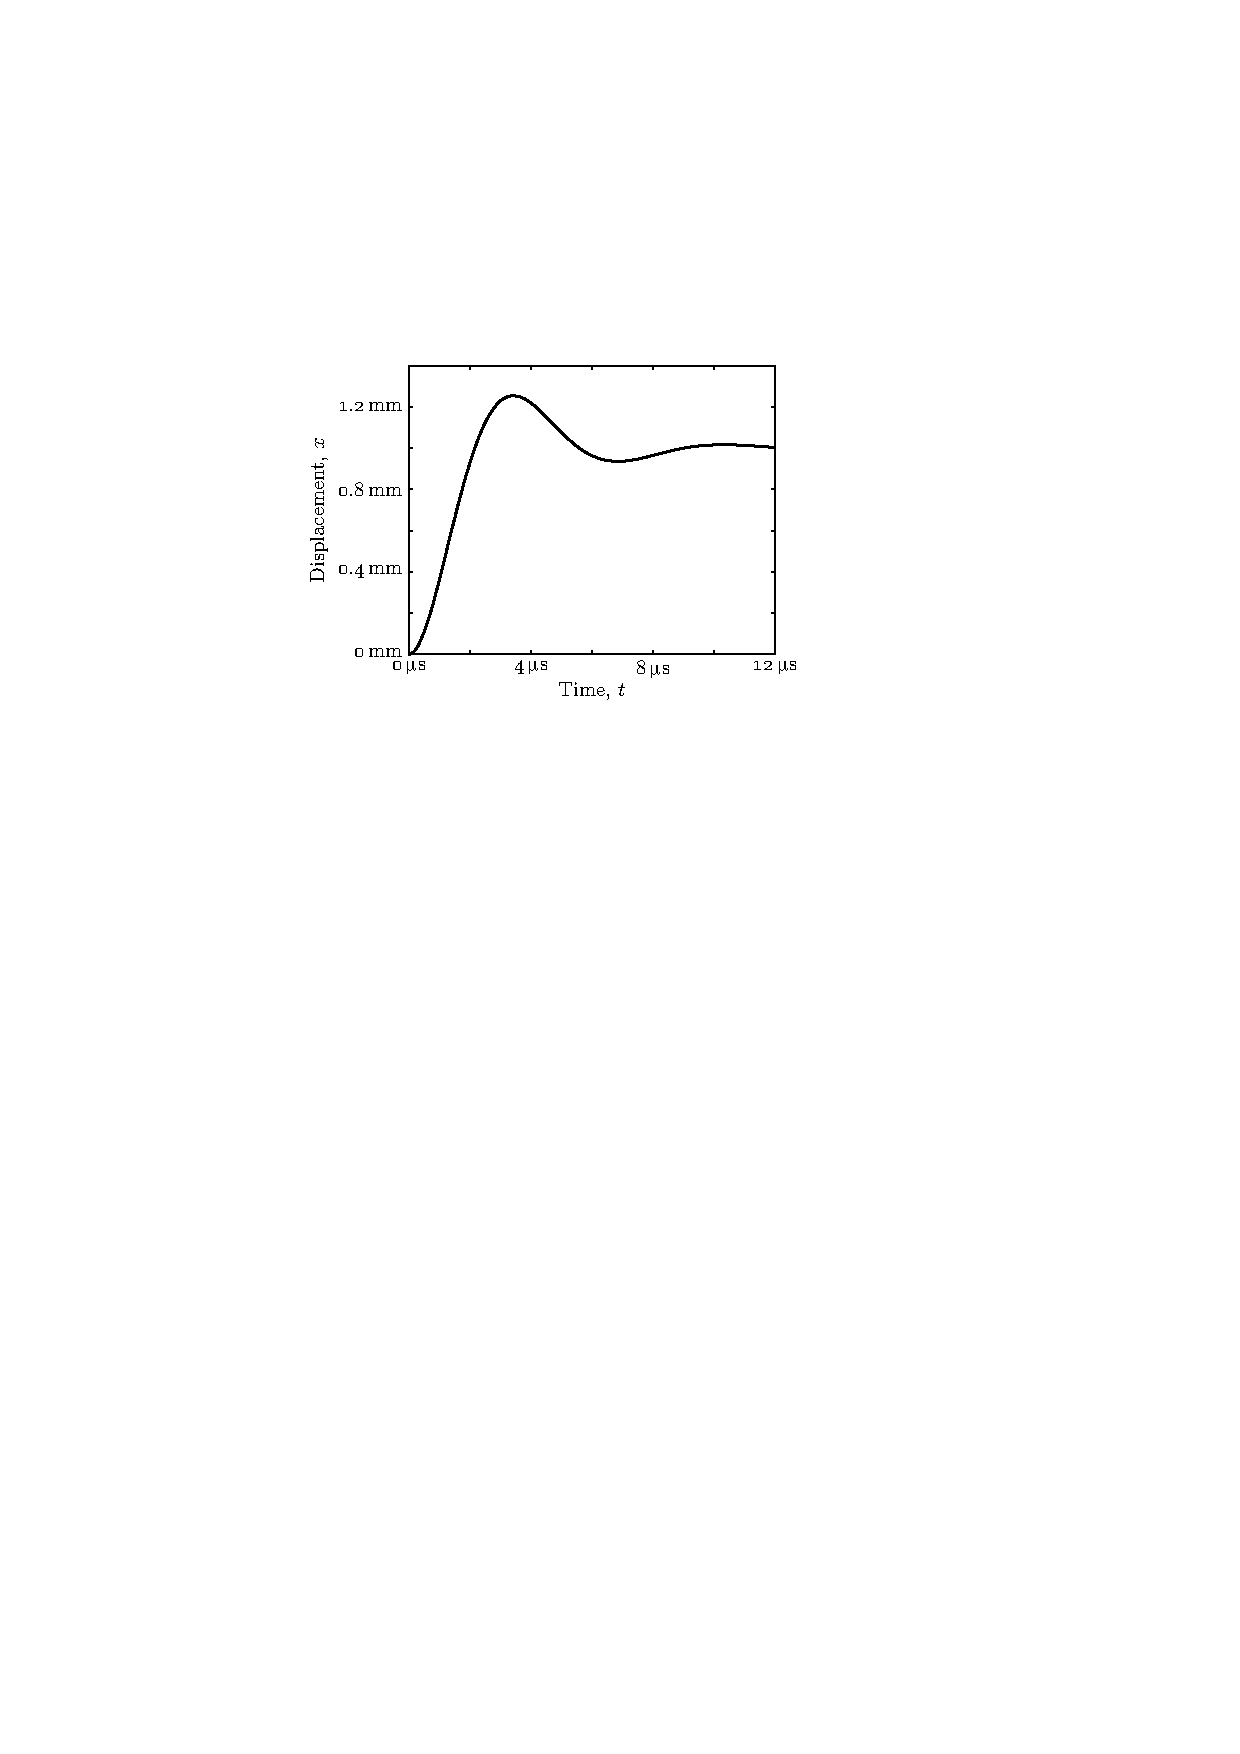
\includegraphics{figs/fig1}}^^A
% \sbox{\tboxb}{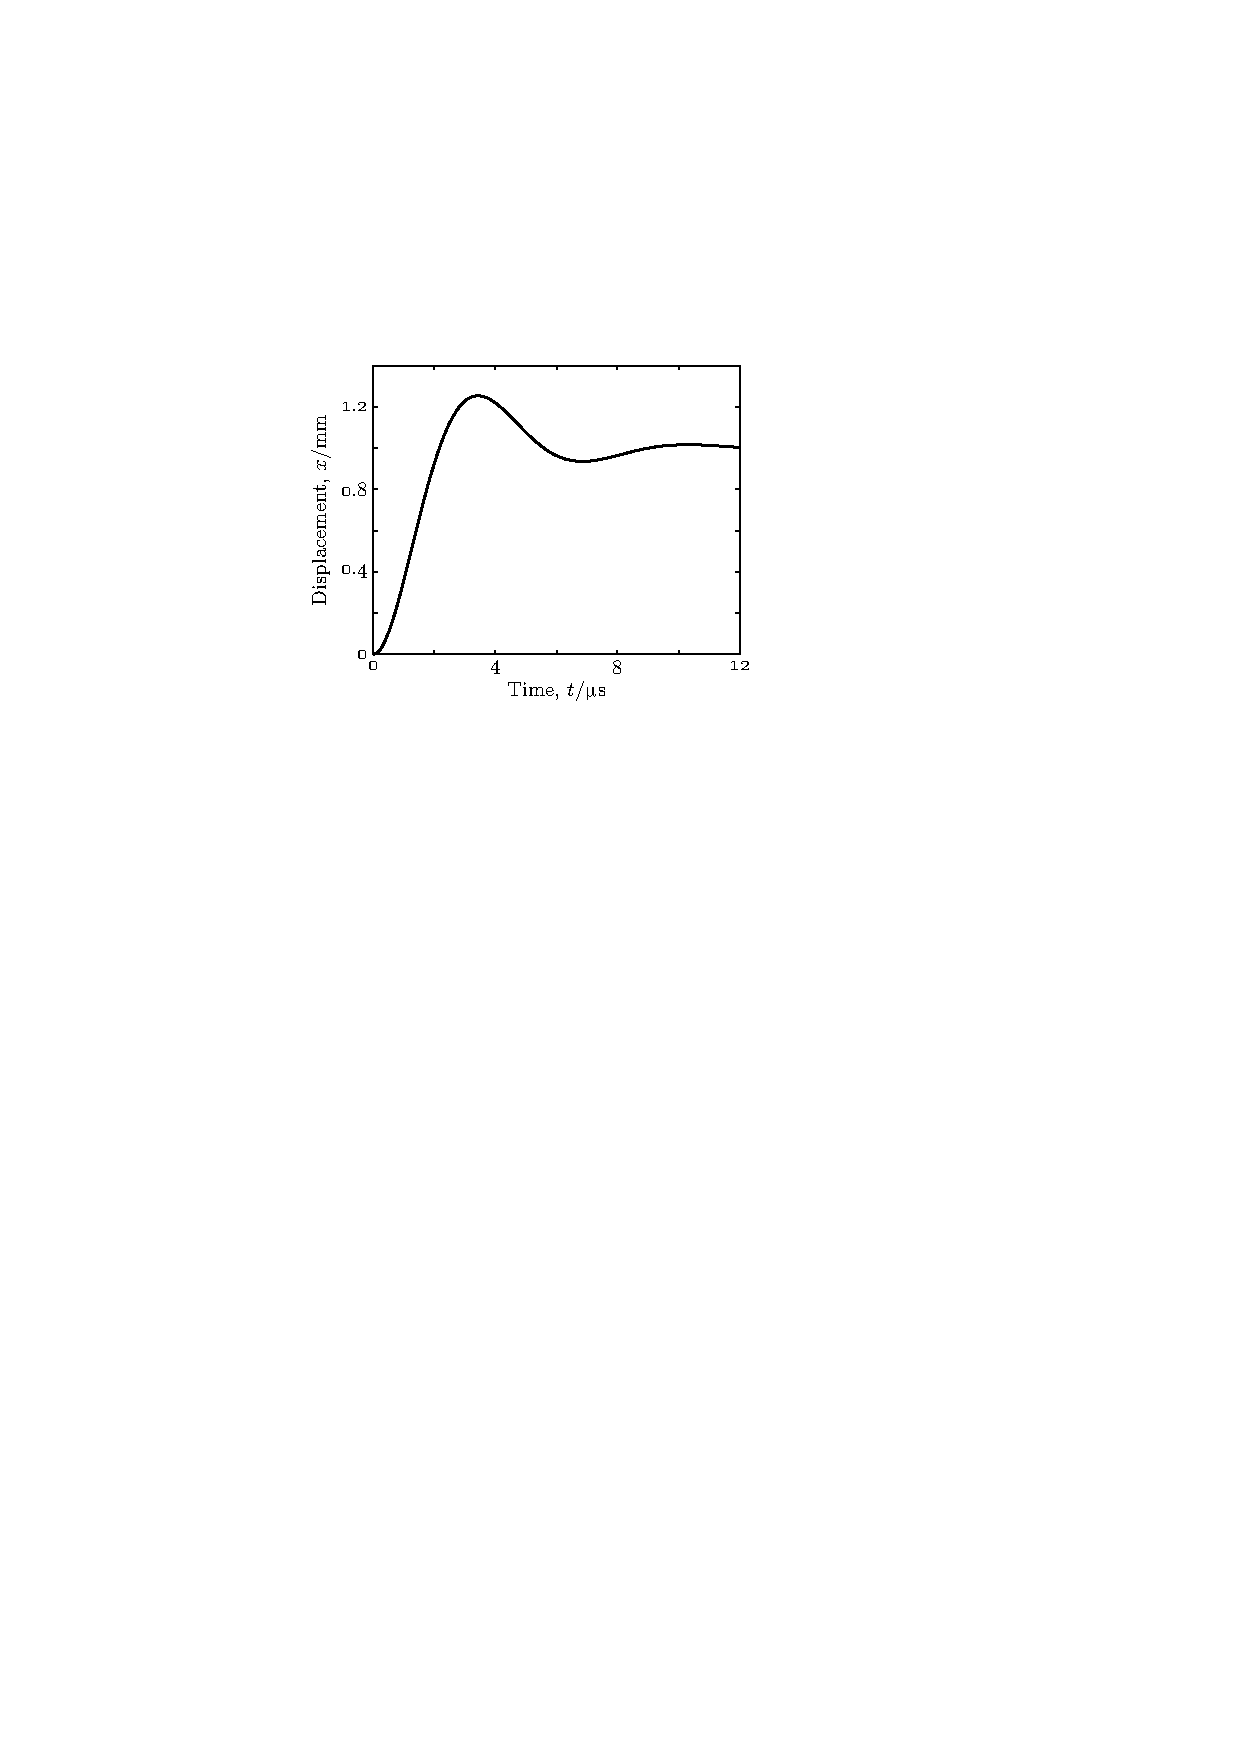
\includegraphics{figs/fig2}}^^A
% \setlength{\tdima}{\wd\tboxa}^^A
% \addtolength{\tdima}{\wd\tboxb}^^A
% \addtolength{\tdima}{1em}^^A
% \centering^^A
% \makebox[0pt][c]{
% \begin{minipage}[t]{\tdima}
%    \begin{minipage}[t]{\wd\tboxa}
%       \usebox{\tboxa}
%       \caption{Units included with the scale of the graph. This
%                form is usually difficult to obtain with most
%                graphing software.}
%       \label{fig:1}
%    \end{minipage}
%    \hfill
%    \begin{minipage}[t]{\wd\tboxb}
%       \usebox{\tboxb}
%       \caption{The graph labels includes the units and the scales
%                 are dimensionless. Notice that there is no
%                 ambiguity with this form of labeling, because
%                 everything makes mathematical sense.}
%        \label{fig:2}
%    \end{minipage}
% \end{minipage}}
% \end{figure}
%
%
% \begin{Item}{Example}
% \end{Item}
% \begin{enumerate}
% \item In the SI, the value of the velocity of light in vacuum is
%       $c = \SI{299792458}{m/s}$ exactly. The number
%       \num{299792458} is the numerical value of $c$ when $c$ is
%       expressed in the unit \SI{}{m/s}, and equals $c/(\SI{}{m/s})$.
%
%       \begin{Item}{Listing}\small
%          |$c = \SI{299792458}{m/s}$|\\
%          |$c/(\SI{}{m/s})$|
%       \end{Item}
%
% \item The ordinate of a graph is labeled $t/\SI{}{\micro s}$,
%       where $t$ is the symbol for time and \SI{}{s} is the unit
%       symbol for second, and has scale marks at \num{0}, \num{4},
%       \num{8}, and \num{12}. If the ordinate
%       value of a point on a curve in the graph is estimated to
%       be \num{3.2}, the corresponding time is ~
%       $t/\SI{}{\micro s}=\num{3.2}$ ~ or ~ $t =\SI{3.2}{\micro s}
%       = \SI{3.6e-6}{s}$. Notice
%       the lack of ambiguity in this form of labelling compared
%       with ``Time $(\SI{}{\micro s})$.'' See figures
%       \ref{fig:1} and \ref{fig:2} for examples.
%
% \item An expression such as $\ln(p/\SI{}{MPa})$, where $p$ is the
%       quantity symbol for pressure and \SI{}{MPa} is the unit symbol
%       for megapascal, is perfectly acceptable because $p/\SI{}{MPa}$
%       is the numerical value of $p$ when $p$ is expressed in the
%       unit \SI{}{MPa} and is simply a number.
%       \begin{Item}{Listing}\small
%          |$\ln(p/\SI{}{MPa})$|
%       \end{Item}
% \end{enumerate}
%
%
%
% \begin{Item}{Notes}
% \end{Item}
% \begin{enumerate}
% \item For the conventions concerning the grouping of digits, see
%       section~\S\ref{sec:digits}.
%
% \item An alternative way of writing $c/(\SI{}{m/s})$ is
%       $\{c\}_{\SI{}{m/s}}$, meaning the numerical value of $c$ when
%       $c$ is expressed in the unit \SI{}{m/s}.
%
%       \begin{Item}{Listing}\small
%          |$\{c\}_{\SI{}{m/s}}$|
%       \end{Item}
% \end{enumerate}
%
%
% \subsection{Space between numerical value and unit symbol}
%
% In the expression for the value of a quantity, the unit symbol is
% placed after the numerical value and a \myemph{space} is left
% between the numerical value and the unit symbol. Note that this
% rule includes the persentage sign \%.
%
% The only exceptions to this rule are for the unit symbols for
% degree, minute, and second for plane angles: \arcdeg, \arcmin, and
% \arcsec, respectively, in which case no space is left between the
% numerical value and the unit symbol.
%
% \begin{Item}{Examples}
%   $x = \SI{10}{mm}$\\
%   $q = \SI{25}{\%}$\\
%   $\theta = \ang{30;22;8}$
% \end{Item}
% \begin{Item}{Listing}\small
%   |$x = \SI{10}{mm}$|\\
%   |$q = \SI{25}{\%}$|\\
%   |$\theta = \ang{30;22;8}$|
% \end{Item}
%
% \noindent This rule means that:
%
% \begin{enumerate}
% \item The symbol \degC\ for the degree Celsius is preceded by a
%       space when one expresses the values of Celsius temperatures.
%
%       \begin{Item}{Example}
%         $t = \SI{30.2}{\degC}$~~
%            \myemph{but not:}~~
%         $t = \num{30.2}\degC$ ~~or~~
%         $t = \num{30.28}\mathrm{{}^{\circ}~C}$
%       \end{Item}
%       \begin{Item}{Listing}\small
%         |$t = \SI{30.2}{\degC}$|
%       \end{Item}
%
% \item Even when the value of a quantity is used in an adjectival
%       sense, a space is left between the numerical value and the
%       unit symbol. (This rule recognizes that unit symbols are not
%       like ordinary words or abbreviations but are mathematical
%       entities, and that the value of a quantity should be
%       expressed in a way that is as independent of language as
%       possible.)
%
%       \begin{Item}{Examples}
%          a \SI{1}{m} end gauge
%              \myemph{but not:}
%          a \num{1}-\SI{}{m} end gauge
%
%          a \SI{10}{kV} resistor
%              \myemph{but not:}
%          a \num{10}-\SI{}{kV} resistor
%       \end{Item}
%
%       However, if there is any ambiguity, the words should be
%       rearranged accordingly. For example, the statement ``the
%       samples were placed in \SI{22}{mL} vials'' should be
%       replaced with the statement ``the samples were placed in
%       vials of volume \SI{22}{mL}.''
%
%       \begin{Item}{Note}
%          When unit names are spelled out, the normal rules of
%          English apply. Thus, for example, ``a roll of
%          \num{35}-millimetre film'' is acceptable.
%       \end{Item}
% \end{enumerate}
%
% \subsection{Clarity in writing values of quantities}
%
% The value of a quantity is expressed as the product of a number
% and a unit (see section~\S\ref{sec:numval}). Thus, to avoid
% possible confusion, this \myemph{Guide} takes the position that
% values of quantities must be written so that it is completely
% clear to which unit symbols the numerical values of the quantities
% belong. Also to avoid possible confusion, this \myemph{Guide}
% strongly recommends that the word ``to'' be used to indicate a
% range of values for a quantity instead of a range dash (that is, a
% long hyphen) because the dash could be misinterpreted as a minus
% sign. (The first of these recommendations once again recognizes
% that unit symbols are not like ordinary words or abbreviations but
% are mathematical entities --- see section~\S\ref{sec:numval}.)
%
% \begin{Item}{Examples}
% \end{Item}
% \begin{tabbing}
% \hskip1pc\=\hskip15pc\=\kill \>
% $\SI{51}{mm}\times\SI{51}{mm}\times\SI{25}{mm}$ \>
%    \myemph{but not:} ~
%    $\num{51}\times\num{51}\times\SI{25}{mm}$ \\[1ex]
%
% \> \SI{225}{nm} to \SI{2400}{nm} or
%    $(\num{225}\text{ to }\num{2400})\,\SI{}{nm}$ \>
%    \myemph{but not:}  ~
%    \num{225} to \SI{2400}{nm}\\[1ex]
%
% \> \SI{0}{\degC} to \SI{100}{\degC} or
%    $(\num{0}\text{ to }\num{100})\,\degC$ \>
%    \myemph{but not:} ~
%    $\SI{0}{\degC} - \SI{100}{\degC}$\\[1ex]
%
% \> \SI{0}{V} to \SI{5}{V} or (\num{0} to \num{5})\,V \>
%    \myemph{but not:} ~
%    $\num{0} - \SI{5}{V}$ \\[1ex]
%
% \> (\num{8.2}, \num{9.0}, \num{9.5}, \num{9.8},
%    \num{10.0})\,\SI{}{GHz} \>
%    \myemph{but not:} ~
%    \num{8.2}, \num{9.0}, \num{9.5}, \num{9.8}, \SI{10.0}{GHz}\\[1ex]
%
% \> $\SI{63.2}{m} \pm \SI{0.1}{m}$ or $(\num{63.2} \pm
%    \num{0.1})\,\SI{}{m}$ \>
%    \myemph{but not:} ~
%    $\num{63.2} \pm \SI{0.1}{m}$ or $\SI{63.2}{m} \pm \num{0.1}$ \\[1ex]
%
% \> $\SI{129}{s} - \SI{3}{s} = \SI{126}{s}$ or
%    $(\num{129}-\num{3})\,\SI{}{s} = \SI{126}{s}$ \>
%    \myemph{but not:} ~
%    $\num{129} - \SI{3}{s} = \SI{126}{s}$
%
% \end{tabbing}
%
% \begin{Item}{Note}
% For the conventions concerning the use of the multiplication sign,
% see section~\S\ref{sec:mult}.
% \end{Item}
%
%^^A==========================================================
%
% \section{Printing Numbers}
%
% \subsection{Typeface for numbers}
%
% Arabic numerals expressing the numerical values of quantities are
% generally printed in lightface (that is, regular) roman type
% irrespective of the type used for the surrounding text. Arabic
% numerals other than numerical values of quantities may be printed
% in lightface or bold italics, or in bold roman type, but lightface
% roman type is usually preferred.
%
% \subsection{Decimal sign or marker}
%
% The sign or marker being used depends very much on the practices
% of a country (and/or language), e.g., in the United States is the
% dot on the line, while in Germany it is the comma.
%
% For numbers less than one, a zero is written before the decimal
% marker. For example, \SI{0.25}{s} is the correct form, not
% \xnum{.25}\,s.
%
% \subsection{Grouping digits}\label{sec:digits}
%
% Because the comma is widely used as the decimal marker, it should
% not be used to separate digits into groups of three (there are
% exceptions for certain countries). Instead, digits should be
% separated into groups of three, counting from the decimal marker
% towards the left and right, by the use of a thin, fixed space.
% However, this practice is not usually followed for numbers having
% only four digits on either side of the decimal marker except when
% uniformity in a table is desired.
% \begin{Item}{Examples}
% \begin{tabbing}
%    \xnum{8012.5947} or \xnum{8\;012.594\;7}~\= \myemph{is highly preferred to:}~~\=\kill
%    \num{76483522}                         \> \myemph{but not:}                 \>\xnum{76{,}483{,}522}\\
%    \num{43279.16829}                      \> \myemph{but not:}                 \>\xnum{43{,}279.168\;29}\\
%   \xnum{8012} or \xnum{8\;012}            \> \myemph{but not:}                 \>\xnum{8{,}012}\\
%    \num{0.4917223}                        \> \myemph{is highly preferred to:}  \>\xnum{0.4917223}\\
%   \xnum{0.5947} or \xnum{0.594\;7}        \> \myemph{but not:}                 \>\xnum{0.59\;47}\\
%   \xnum{8012.5947} or \xnum{8\;012.594\;7}\> \myemph{but not:}                 \>\xnum{8\;012.5947} or \xnum{8012.594\;7}
% \end{tabbing}
% \end{Item}
%
% \begin{Item}{Note}
%    The practice of using a space to group digits is not usually
%    followed in certain specialized applications, such as engineering
%    drawings and financial statements.
% \end{Item}
%
%
% \subsection{Multiplying numbers}\label{sec:mult}
%
% When the dot is used as the decimal marker (USA convention), the
% preferred sign for the multiplication of numbers or values of
% quantities is a cross (that is, multiplication sign) ($\times$),
% not a half-high (that is, centered) dot ($\cdot$).
%
% \begin{Item}{Examples}
% \begin{tabular}[t]{@{}lll@{}}
%  $\num{25}\times\num{60.5}$       &\myemph{but not:}& $\num{25}\cdot\num{60.5}$\\
%  $\SI{53}{m/s}\times\SI{10.2}{s}$ &\myemph{but not:}& $\SI{53}{m/s}\cdot\SI{10.2}{s}$\\
%  $\num{15}\times\SI{72}{kg}$      &\myemph{but not:}& $\num{15}\cdot\SI{72}{kg}$\\
% \end{tabular}
% \end{Item}
%
%
% \begin{Item}{Notes}
% \end{Item}
% \begin{enumerate}
% \item When the comma is used as the decimal marker, the preferred
%       sign for the multiplication of numbers is the half-high dot
%       (German convention).
%       \begin{Ipara}[\normalsize]
%       \xnum{3{,}645\;98 \cdot 10^2} ~ or ~
%       \xnum{2{,}58 \cdot 31{,}2}
%       \end{Ipara}
%       The comma is also used together with the cross for the
%       multiplication of values of quantities (South African Convention).
%       \begin{Ipara}[\normalsize]
%       \xnum{3{,}645\;98 {\times} 10^2} ~ or ~
%       \xnum{2{,}58 \times 31{,}2}
%       \end{Ipara}
%
% \item The multiplication of quantity symbols (or numbers in
% parentheses or values of quantities in parentheses) may be
% indicated in one of the following ways: $ab$, $a\;b$, $a\cdot b$,
% $a\times b$.
% \end{enumerate}
%
%
%^^A=================================================================
% \StopEventually{\PrintChanges\PrintIndex}
% \clearpage
% \part{Implementation: \pkg{SIstyle}}
%
%    \begin{macrocode}
%<*package>
%    \end{macrocode}
%
%    \section{Utilities}
%
%    We need the \cmd{\text} command from the \AmS\ package
%    \pkg{amstext} for the typesetting of text in math mode.
%    \begin{macrocode}
\RequirePackage{amstext}
%    \end{macrocode}
%
%    \subsection{Test for $\varepsilon$-\TeX}
%    \begin{macrocode}
\newif\ifSI@eTeX
\SI@eTeXfalse
\ifx\eTeXversion\@undefined
\else
  \ifx\eTeXversion\relax
  \else
    \ifnum\eTeXversion>\z@
      \SI@eTeXtrue
    \fi
  \fi
\fi
%    \end{macrocode}
%
%    \subsection{Test for empty argument}
%
%    \begin{macro}{\SI@ifempt}
%    Test for a empty argument (Wilson, Arseneau in
%    \pkg{ifmtarg.sty}).\\
%    Usage: \cmd{\SI@ifempt}\marg{arg}\marg{true}\marg{false}
%
%    \begin{macrocode}
\begingroup
   \catcode`\Q=3
   \long\gdef\SI@ifempt#1{\SI@xifempt#1QQ\@secondoftwo\@firstoftwo\@nil}
   \long\gdef\SI@xifempt#1#2Q#3#4#5\@nil{#4}
\endgroup
%    \end{macrocode}
%    \end{macro}
%
%    \subsection{Font test commands}
%
%    \begin{macro}{\GetMathFontFams}
%    There exists no hook to test for the current active
%    math font. Get the different families at the beginning
%    of the document. We only look for \cmd{\mathsf} and
%    \cmd{\mathtt}. The others are set with the default
%    math font (\cmd{\mathrm}).
%    \begin{macrocode}
 \newcommand{\GetMathFontFams}{%
    \sbox{0}{$%
       \@ifundefined{mathsf}
          {\global\chardef\SI@sffam=99}%
          {\mathsf{\global\chardef\SI@sffam=\fam}}%
       \@ifundefined{mathtt}
          {\global\chardef\SI@ttfam=99}%
          {\mathtt{\global\chardef\SI@ttfam=\fam}}%
       $}%
  }
%    \end{macrocode}
%    \end{macro}
%    \begin{macrocode}
\AtBeginDocument{\GetMathFontFams}
%    \end{macrocode}
%
%    \begin{macro}{\IfTbold}
%    Test if bold text (\cmd{\bfseries} or \cmd{\bxseries}) is
%    active.\\
%    Usage: \cmd{\IfTbold}\marg{true}\marg{false}
%    \begin{macrocode}
\newcommand{\IfTbold}[2]{%
   \if b\expandafter\@car\f@series\@nil%
      #1\else #2\fi}
%    \end{macrocode}
%    \end{macro}
%
%    \begin{macro}{\IfMbold}
%    Test if \cmd{\boldmath} is active.
%    Usage: \cmd{\IfMbold}\marg{true}\marg{false}
%    \begin{macrocode}
\newcommand{\IfMbold}[2]{%
   \edef\temp@bm{bold}%
   \ifx\math@version\temp@bm
      #1\else #2\fi}
%    \end{macrocode}
%    \end{macro}
%
%
%    \subsection{Font user setup commands}
%
%    \begin{macro}{\SIobeybold}
%    User flag to obey bold text and math bold setting for
%    SI units and numbers.
%    \begin{macrocode}
\newif\ifSIobeybold
\SIobeyboldfalse
%    \end{macrocode}
%    \end{macro}
%
%    \begin{macro}{\SI@mathrm}
%    \begin{macro}{\SI@mathsf}
%    \begin{macro}{\SI@mathtt}
%    \begin{macro}{\SImathrm}
%    \begin{macro}{\SImathsf}
%    \begin{macro}{\SImathtt}
%    Make user commands to override \cmd{\mathrm}, \cmd{\mathsf}
%    and \cmd{\mathtt},
%    \begin{macrocode}
\newcommand*{\SI@mathrm}{\mathrm}
\newcommand*{\SI@mathsf}{\mathsf}
\newcommand*{\SI@mathtt}{\mathtt}
\newcommand*{\SImathrm}[1]{\renewcommand*{\SI@mathrm}{#1}}
\newcommand*{\SImathsf}[1]{\renewcommand*{\SI@mathsf}{#1}}
\newcommand*{\SImathtt}[1]{\renewcommand*{\SI@mathtt}{#1}}
%    \end{macrocode}
%    \end{macro}
%    \end{macro}
%    \end{macro}
%    \end{macro}
%    \end{macro}
%    \end{macro}
%
%
%    \begin{macro}{\SIdefaultMfam}
%    \begin{macro}{\SI@defaultMfam}
%    The default upright math font for typesetting SI units. This
%    is normally the \cmd{\mathrm} command, but the user may select
%    a different font.
%    \begin{macrocode}
\newcommand*{\SI@defaultMfam}{\SI@mathrm}
\newcommand*{\SIdefaultMfam}[1]{\renewcommand*{\SI@defaultMfam}{#1}}
%    \end{macrocode}
%    \end{macro}
%    \end{macro}
%    \begin{macro}{\SIdefaultNfam}
%    \begin{macro}{\SI@defaultNfam}
%    The default upright math font for typesetting numbers. This
%    is normally the \cmd{\mathrm} command, but the user may select
%    a different font, for example \cmd{\mathnormal} to obtain
%    old-style digits.
%    \begin{macrocode}
\newcommand*{\SI@defaultNfam}{\SI@mathrm}
\newcommand*{\SIdefaultNfam}[1]{\renewcommand*{\SI@defaultNfam}{#1}}
%    \end{macrocode}
%    \end{macro}
%    \end{macro}
%
%    \begin{macro}{\SIdefaultTfam}
%    \begin{macro}{\SI@defaultTfam}
%    The default text font for units set inside a \cmd{\mbox},
%    such as symbols from the \pkg{textcomp} package. It sets the
%    font when the surrounding text font is not \cmd{\sffamily} or
%    \cmd{\ttfamily} or if it is set inside display math.
%    \begin{macrocode}
\newcommand*{\SI@defaultTfam}{\rmfamily}
\newcommand*{\SIdefaultTfam}[1]{\renewcommand*{\SI@defaultTfam}{#1}}
%    \end{macrocode}
%    \end{macro}
%    \end{macro}
%
%    \begin{macro}{\SIupmath}
%    This command set units and numbers in an upright font.
%    When called inside a normal text paragraph or inside
%    inline math |$...$|, it will follow the surrounding
%    text font: sansserif or typewrite otherwise it will
%    default to the roman font. Inside display math it will
%    follows the active math font.
%
%    The prerequisite to toggle the \cmd{\boldmath} math version
%    results in setting the argument inside the \AmS\ \cmd{\text}
%    command. It has the added benefit of scaling with the active
%    math style.
%
%    Usage: \cmd{\SIupmath}\oarg{math font}\marg{argument}
%
%    \begin{macro}{\ifupmath}
%    Flag to indicate whether we are inside \cmd{\SIupmath}.
%    \begin{macrocode}
\newif\ifupmath
\upmathfalse
%    \end{macrocode}
%    \begin{macrocode}
\newcommand*{\SIupmath}[2][\SI@defaultMfam]{%
\begingroup
   \upmathtrue
   \edef\temp@sf{\sfdefault}%
   \edef\temp@tt{\ttdefault}%
   \let\SI@bold=\relax
   \ifmmode
      \ifdim\displaywidth>0pt\relax%--- DISPLAY MATH ------------
         \ifnum\the\fam=\SI@sffam
            \let\SI@mfam=\SI@mathsf
            \let\SI@tfam=\sffamily
         \else \ifnum\the\fam=\SI@ttfam
            \let\SI@mfam=\SI@mathtt
            \let\SI@tfam=\ttfamily
         \else
            \let\SI@mfam=#1%
            \let\SI@tfam=\SI@defaultTfam
         \fi\fi
         \IfMbold{\def\SI@bold{\bfseries}}%
                 {\def\SI@bold{\mdseries}}%
      \else%--- INLINE MATH ----------
         \ifx\f@family\temp@sf
            \let\SI@mfam=\SI@mathsf
            \let\SI@tfam=\sffamily
         \else\ifx\f@family\temp@tt
            \let\SI@mfam=\SI@mathtt
            \let\SI@tfam=\ttfamily
         \else
            \let\SI@mfam=#1%
            \let\SI@tfam=\SI@defaultTfam
         \fi\fi
         \IfTbold{\def\SI@bold{\boldmath}}%
                 {\def\SI@bold{\unboldmath}}%
      \fi
   \else%----- NORMAL TEXT --------------
      \ifx\f@family\temp@sf
         \let\SI@mfam=\SI@mathsf
         \let\SI@tfam=\sffamily
      \else\ifx\f@family\temp@tt
         \let\SI@mfam=\SI@mathtt
         \let\SI@tfam=\ttfamily
      \else
         \let\SI@mfam=#1%
         \let\SI@tfam=\SI@defaultTfam
      \fi\fi
      \IfTbold{\def\SI@bold{\boldmath}}%
              {\def\SI@bold{\unboldmath}}%
   \fi%----- END OF TEST --------------
   \text{%
      \ifSIobeybold\SI@bold\else\unboldmath\mdseries\fi
      \upshape\SI@tfam
      $\SI@mfam{#2}$}%
\endgroup
\check@mathfonts}
%    \end{macrocode}
%    \end{macro}
%    \end{macro}
%
%    \begin{macro}{\ensureupmath}
%    A user command to use the \cmd{\SIupmath} command.
%    \begin{macrocode}
\DeclareRobustCommand{\ensureupmath}{%
   \ifupmath
      \expandafter\@firstofone
   \else
      \expandafter\SIupmath
   \fi}
%    \end{macrocode}
%    \end{macro}
%
%
%    \section{Typeset Numbers}
%
%    \subsection{Setup for typesetting numbers}
%
%    \begin{macro}{\SIdecimalsign}
%    \begin{macro}{\SI@decsign}
%    User command to set decimal sign.
%    \begin{macrocode}
\newcommand*{\SI@decsign}{{.}}
\newcommand*{\SIdecimalsign}[1]{\renewcommand*{\SI@decsign}{{#1}}}
%    \end{macrocode}
%    \end{macro}
%    \end{macro}
%
%    \begin{macro}{\SIthousandsep}
%    \begin{macro}{\SI@thousandsep}
%    User command to set thousands separator.
%    \begin{macrocode}
\newcommand*{\SI@thousandsep}{{\,}}
\newcommand*{\SIthousandsep}[1]{\renewcommand*{\SI@thousandsep}{{#1}}}
%    \end{macrocode}
%    \end{macro}
%    \end{macro}
%
%    \begin{macro}{\SIproductsign}
%    \begin{macro}{\SI@prod}
%    User command to set product sign.
%    \begin{macrocode}
\newcommand*{\SI@prod}{\ensuremath{{}\times{}}}
\newcommand*{\SIproductsign}[1]{\renewcommand*{\SI@prod}{\ensuremath{{}#1{}}}}
%    \end{macrocode}
%    \end{macro}
%    \end{macro}
%
%    \begin{macro}{\ifSIgroupfour}
%    User flag for the grouping of four digits.
%    \begin{macrocode}
\newif\ifSIgroupfour
\SIgroupfourtrue
%    \end{macrocode}
%    \end{macro}
%
%
%    \subsection{Number parser}
%
%    \begin{macro}{\SI@num}
%     Main command for typesetting numbers. Zap all input spaces and
%     make E's lowercase.
%    \begin{macrocode}
\def\SI@num#1{%
   \SI@ifempt{#1}{}{%
      \edef\SI@tmpa{\lowercase{\noexpand\SI@@num{\zap@space#1 \@empty}}}%
      \SI@tmpa}}
%    \end{macrocode}
%    \end{macro}
%
%    \begin{macro}{\SI@@num}
%    \begin{macro}{\SI@numsplit}
%    Split of the exponential part (Downes, Oberdiek on c.t.t)
%    \begin{macrocode}
\def\SI@@num#1{\SI@numsplit#1ee\SI@numexp\SI@realp\@empty}
\def\SI@numsplit#1e#2e#3#4#5{#4{#1}{#2}}
%    \end{macrocode}
%    \end{macro}
%    \end{macro}
%
%    \begin{macro}{\SI@p@tst}
%    \begin{macro}{\SI@m@tst}
%    Temporaries to test for $+$ and $-$.
%    \begin{macrocode}
\def\SI@p@tst{+}
\def\SI@m@tst{-}
%    \end{macrocode}
%    \end{macro}
%    \end{macro}
%
%    \begin{macro}{\SI@numexp}
%    Type the exponent if the argument contains an ``E'' or ``e''.
%    \begin{macrocode}
\def\SI@numexp#1#2{%
   \SI@ifempt{#1}{}{%
      \def\SI@tmpb{#1}%
      \ifx\SI@tmpb\SI@p@tst\ensuremath{+}\else
      \ifx\SI@tmpb\SI@m@tst\ensuremath{-}\else
         \SI@realp{#1}{}\SI@prod%
      \fi\fi}%
   \ifmmode
     10^{\SI@realp{#2}{}}%
   \else
     10\textsuperscript{\SI@realp{#2}{}}%
   \fi}
%    \end{macrocode}
%    \end{macro}
%
%
%    \begin{macro}{\SI@realp}
%    \begin{macro}{\SI@realpsplit}
%    Split of the integer and decimal part (for decimal point).
%    \begin{macrocode}
\def\SI@realp#1#2{\SI@realpsplit#1..\SI@realfrc\SI@realc\@empty}
\def\SI@realpsplit#1.#2.#3#4#5{#4{#1}{#2}}
%    \end{macrocode}
%    \end{macro}
%    \end{macro}
%
%    \begin{macro}{\SI@realc}
%    \begin{macro}{\SI@realcsplit}
%    Split of the integer and decimal part (for decimal comma).
%    \begin{macrocode}
\def\SI@realc#1#2{\SI@realcsplit#1,,\SI@realfrc\SI@signedint\@empty}
\def\SI@realcsplit#1,#2,#3#4#5{#4{#1}{#2}}
%    \end{macrocode}
%    \end{macro}
%    \end{macro}
%
%
%    \begin{macro}{\SI@realfrc}
%    Type the number if it contains a fraction part. Insert a zero
%    if the integer is empty (no sign either).
%    \begin{macrocode}
\def\SI@realfrc#1#2{%
   \SI@ifempt{#1}{\SI@int{0}}%
                 {\SI@signedint{#1}{}}%
   \SI@decsign\SI@dec{#2}}
%    \end{macrocode}
%    \end{macro}
%
%    \begin{macro}{\SI@signedint}
%    Split the plus and minus from the integer.
%    \begin{macrocode}
\def\SI@signedint#1#2{\SI@@signedint#1 }
\def\SI@@signedint#1#2 {%
  \if +#1\ensuremath{+}%
      \SI@ifempt{#2}{\SI@int{0}}{\SI@int{#2}}%
  \else
  \if -#1\ensuremath{-}%
      \SI@ifempt{#2}{\SI@int{0}}{\SI@int{#2}}%
  \else
  \SI@int{#1#2}\fi \fi}
%    \end{macrocode}
%    \end{macro}
%
%
%    \begin{macro}{\SI@not@v}
%    \begin{macro}{\SI@@not@v}
%    Test for a fifth digit.
%    \begin{macrocode}
\def\SI@not@v#1{\SI@@not@v#1\@empty\@empty\@empty\@empty\@empty\@nil}
\def\SI@@not@v#1#2#3#4#5\@nil{%
   \ifx\@empty#5\@empty
      \expandafter\@firstoftwo
   \else
      \expandafter\@secondoftwo
   \fi}
%    \end{macrocode}
%    \end{macro}
%    \end{macro}
%
%
%    \begin{macro}{\SI@int}
%    Set the integer. If \cmd{\ifSIgroup} is true and the number has
%    four or less digits, then set the number. Otherwise pass it
%    on to the formatting command.
%    \begin{macrocode}
\def\SI@int#1{%
   \ifSIgroupfour
      \SI@not@v{#1}{#1}{\SI@intfmt{}#1\@empty\@empty\@empty}%
   \else
      \SI@intfmt{}#1\@empty\@empty\@empty%
   \fi}
%    \end{macrocode}
%    \end{macro}
%
%
%    \begin{macro}{\SI@intfmt}
%    \begin{macro}{\SI@intfmtafterfi}
%    \begin{macro}{\SI@addthousandsep}
%    Finally typeset the integer in groups of three. (From a macro
%    to typeset Dollar amounts by Donald Arseneau on c.t.t.)
%    \begin{macrocode}
\def\SI@intfmt#1#2#3#4{%
  \ifx\@empty#2\@empty%
    \SI@addthousandsep#1\relax
  \else
    \ifx\@empty#3\@empty%
      \SI@addthousandsep\@empty\@empty#1#2\relax
    \else
      \ifx\@empty#4\@empty%
        \SI@addthousandsep\@empty#1#2#3\relax
      \else
        \SI@intfmtafterfi{#1#2#3#4}%
      \fi
    \fi
  \fi}
%    \end{macrocode}
%
%    \begin{macrocode}
\def\SI@intfmtafterfi#1\fi\fi\fi{\fi\fi\fi\SI@intfmt{#1}}
%    \end{macrocode}
%
%    \begin{macrocode}
\def\SI@addthousandsep#1#2#3#4{#1#2#3%
  \if\relax#4\relax
  \else
    \SI@thousandsep\expandafter\SI@addthousandsep\expandafter#4%
  \fi}
%    \end{macrocode}
%    \end{macro}
%    \end{macro}
%    \end{macro}
%
%    \begin{macro}{\SI@dec}
%    \begin{macro}{\SI@decfmt}
%     Set the decimal part (from \pkg{frenchb.ldf} by by Johannes L. Braams)
%    \begin{macrocode}
\def\SI@dec#1{%
   \ifSIgroupfour
      \SI@not@v{#1}{#1}{\SI@decfmt#1\@empty\@empty\@empty\@empty}%
   \else
      \SI@decfmt#1\@empty\@empty\@empty\@empty%
   \fi}
%    \end{macrocode}
%
%    \begin{macrocode}
\def\SI@decfmt#1#2#3#4{#1#2#3%
  \ifx\@empty#4\@empty%
  \else
    \SI@thousandsep\expandafter\SI@decfmt\expandafter#4%
  \fi}
%    \end{macrocode}
%    \end{macro}
%    \end{macro}
%
%
%
%
%    \subsection{Number commands}
%
%    \begin{macro}{\SInum}
%    Command to typeset a number in upright math font
%    with \cmd{\SIupmath}
%    \begin{macrocode}
\newcommand*{\SInum}[1]{{%
   \let\SI@unitdot=\pnt%
   \SIupmath[\SI@defaultNfam]{\SI@num{#1}}}}
%    \end{macrocode}
%    \end{macro}
%
%    \begin{macro}{\num}
%    The robust user command to typeset a number.
%    The starred form gives a number in the normal active
%    font.
%    \begin{macrocode}
\DeclareRobustCommand*{\num}{\@ifstar{\SI@num}{\SInum}}
%    \end{macrocode}
%    \end{macro}
%
%
%    \section{Typesetting Angles}
%
%
%    \begin{macro}{\ang}
%    \begin{macro}{\SI@ang}
%    \begin{macro}{\SI@@ang}
%    \begin{macro}{\SI@ang@xii}
%    \begin{macro}{\SI@@ang@xii}
%    \begin{macro}{\SI@ang@xiii}
%    \begin{macro}{\SI@@ang@xiii}
%    The robust user command to typeset angles. Note that we
%    have to make provisions for packages such as French that
%    make the semicolon (;) active
%    \begin{macrocode}
\ifSI@eTeX
    \DeclareRobustCommand{\ang}{%
        \begingroup
            \catcode`;=12\relax
            \catcode`@=11\relax
            \SI@ang}
    \def\SI@ang#1{%
            \scantokens{\SI@@ang#1;;;\@nil}%
        \endgroup}
    \def\SI@@ang#1;#2;#3;#4\@nil{%
        \SI@@@ang{#1}{#2}{#3}}%
\else
    \DeclareRobustCommand{\ang}[1]{%
        \@nameuse{SI@ang@\romannumeral\catcode`\;}{#1}}%
    \begingroup
        \catcode`\;=12\relax
        \gdef\SI@ang@xii#1{\SI@@ang@xii#1;;;\@nil}
        \gdef\SI@@ang@xii#1;#2;#3;#4\@nil{\SI@@@ang{#1}{#2}{#3}}
        \catcode`\;=\active\relax
        \gdef\SI@ang@xiii#1{\SI@@ang@xiii#1;;;\@nil}
        \gdef\SI@@ang@xiii#1;#2;#3;#4\@nil{\SI@@@ang{#1}{#2}{#3}}
    \endgroup
\fi
%    \end{macrocode}
%    \end{macro}
%    \end{macro}
%    \end{macro}
%    \end{macro}
%    \end{macro}
%    \end{macro}
%    \end{macro}
%
%    \begin{macro}{\SI@degs}
%    \begin{macro}{\SI@mins}
%    \begin{macro}{\SI@secs}
%    \begin{macro}{\SI@@@ang}
%    Scratch commands to hold definitions and typeset angles.
%    \begin{macrocode}
\let\SI@degs=\relax
\let\SI@mins=\relax
\let\SI@secs=\relax
%    \end{macrocode}
%    \begin{macrocode}
\newcommand*{\SI@@@ang}[3]{{%
   \SI@ifempt{#3}{}{\def\SI@secs{\SInum{#3}\SIupmath{\arcsec}}%
                    \def\SI@mins{\SInum{0}\SIupmath{\arcmin}}%
                    \def\SI@degs{\SInum{0}\SIupmath{\arcdeg}}}%
   \SI@ifempt{#2}{}{\def\SI@mins{\SInum{#2}\SIupmath{\arcmin}}%
                    \def\SI@degs{\SInum{0}\SIupmath{\arcdeg}}}%
   \SI@ifempt{#1}{}{\def\SI@degs{\SInum{#1}\SIupmath{\arcdeg}}}%
   \SI@degs\SI@mins\SI@secs}}
%    \end{macrocode}
%    \end{macro}
%    \end{macro}
%    \end{macro}
%    \end{macro}
%
%
%     \section{Typesetting Units}
%     \subsection{Unit setup commands}
%
%    \begin{macro}{\SIunitsep}
%    \begin{macro}{\SI@unitsep}
%    User command to set unit separation width from the number.
%    \begin{macrocode}
\newcommand*{\SI@unitsep}{\,}
\newcommand*{\SIunitsep}[1]{\renewcommand*{\SI@unitsep}{#1}}
%    \end{macrocode}
%    \end{macro}
%    \end{macro}
%
%    \begin{macro}{\SIunitspace}
%    \begin{macro}{\SI@unitspace}
%    User command to set the spacing between units when
%    ``\tlde'' is issued.
%    \begin{macrocode}
\newcommand*{\SI@unitspace}{\,}
\newcommand*{\SIunitspace}[1]{\renewcommand*{\SI@unitspace}{#1}}
%    \end{macrocode}
%    \end{macro}
%    \end{macro}
%
%    \begin{macro}{\SIunitdot}
%    \begin{macro}{\SI@unitdot}
%    User command to set the unit dot when ``.'' is
%    given between units.
%    \begin{macrocode}
\newcommand*{\SI@unitdot}{{\cdot}}
\newcommand*{\SIunitdot}[1]{\renewcommand*{\SI@unitdot}{#1}}
%    \end{macrocode}
%    \end{macro}
%    \end{macro}
%
%    \begin{macro}{\pnt}
%    Supply \cmd{\pnt}  command for ``.'' in mathmode.
%    Define the point ``.'' as a command when active
%    (|\mathcode`.="8000|) inside math environment.
%    \begin{macrocode}
\DeclareMathSymbol{\pnt}{\mathord}{letters}{58}   %(\pnt = .)
{\catcode`\.=13 \gdef.{\SI@unitdot}}
%    \end{macrocode}
%    \end{macro}
%
%
%    \subsection{Commands for units}
%
%    \begin{macro}{\SIunit}
%    Command that sets the environment for typesetting units.
%    The ``.'' is made active and the ``\tlde'' is redefined.
%    \begin{macrocode}
\newcommand*{\SIunit}[1]{%
\begingroup%
    \mathcode`.="8000%
    \def~{\SI@unitspace}%
    \SIupmath{#1}%
\endgroup}
%    \end{macrocode}
%    \end{macro}
%
%    \begin{macro}{\SI}
%    Command to typeset numbers with units.
%
%    Usage: \cmd{\SI}\marg{number}\marg{unit}
%    \begin{macrocode}
\DeclareRobustCommand*{\SI}[2]{%
   \SI@ifempt{#1}{}{\SInum{#1}\SI@unitsep}%
   \SIunit{#2}}
%    \end{macrocode}
%    \end{macro}
%
%    \section{Additional Units}
%
%    \noindent
%    Additional non Latin user symbols are defined:
%    \begin{macrocode}
\AtBeginDocument{%
    \@ifpackageloaded{textcomp}{%
         \providecommand*{\micro}{\ensureupmath{\mbox{\textmu}}}%
         \providecommand*{\ohm}{\ensureupmath{\mbox{\textohm}}}%
         \providecommand*{\degC}{\ensureupmath{\mbox{\textcelsius}}}%
         \providecommand*{\degF}{\ensureupmath{\mbox{\textdegree F}}}%
         \providecommand*{\arcdeg}{\ensureupmath{\mbox{\textdegree}}}%
         \providecommand*{\angstrom}{\ensureupmath{\mbox{\capitalring{A}}}}%
    }{%
         \providecommand*{\micro}{\ensureupmath{\mu}}%
         \providecommand*{\ohm}{\ensureupmath{\Omega}}%
         \providecommand*{\degC}{%
             \ensureupmath{{}^{\circ}\kern-\scriptspace C}}%
         \providecommand*{\degF}{%
             \ensureupmath{{}^{\circ}\kern-\scriptspace F}}%
         \providecommand*{\arcdeg}{\ensureupmath{{}^{\circ}}}%
         \providecommand*{\angstrom}{\ensureupmath{\mbox{\AA}}}%
    }%
   \providecommand*{\arcmin}{\ensureupmath{{}^{\prime}}}%
   \providecommand*{\arcsec}{\ensureupmath{{}^{\prime\prime}}}%
}
%    \end{macrocode}
%
%    \section{Locales}
%    \subsection{Macros}
%
%    Temporary tokens.
%    \begin{macrocode}
\newtoks\ttoks@A
\newtoks\ttoks@B
%    \end{macrocode}
%
%    \begin{macro}{\SIstyle}
%    The main command to activate a spesific style.
%    \begin{macrocode}
\newcommand{\SIstyle}[1]{%
   \@ifundefined{SIstyle#1}%
      {\PackageError{SIstyle}{Style `#1' is not defined}%
                           {See SIstyle package documentation}}%
      {\@nameuse{SIstyle#1}}}
%    \end{macrocode}
%    \end{macro}
%
%    \begin{macro}{\AddToSIstyle}
%    \begin{macro}{\SI@s@addto@stl}
%    \begin{macro}{\SI@addto@stl}
%    Append the command list in |#2| to the style command |\SIstyle#1|.
%    The starred form clears the list before appending.
%    \begin{macrocode}
\newcommand{\AddToSIstyle}{%
   \@ifstar{\SI@s@addto@stl}{\SI@addto@stl}}
%    \end{macrocode}
%
%    \begin{macrocode}
\newcommand{\SI@s@addto@stl}[1]{%
   \expandafter\let\csname SIstyle#1\endcsname\relax
   \SI@addto@stl{#1}}
%    \end{macrocode}
%
%    \begin{macrocode}
\newcommand{\SI@addto@stl}[2]{%
   \expandafter\SI@addto@list\csname SIstyle#1\endcsname{#2}}
%    \end{macrocode}
%    \end{macro}
%    \end{macro}
%    \end{macro}
%    \begin{macrocode}
\@onlypreamble\AddToSIstyle
%    \end{macrocode}
%
%    \begin{macro}{\SIstyleToLang}
%    Links a locale to the \pkg{babel} language changing
%    |\extras|\meta{lang}.
%
%    \begin{macrocode}
\newcommand*{\SIstyleToLang}[2]{%
   \expandafter\SI@addto@list
      \csname extras#1\expandafter\endcsname
      \csname SIstyle#2\endcsname}
%    \end{macrocode}
%    \begin{macrocode}
\@onlypreamble\SIstyleToLang
%    \end{macrocode}
%    \end{macro}
%
%    \begin{macro}{\SI@addto@list}
%    The general macro to append to a list
%    (stolen for \pkg{varioref}).
%
%    \begin{macrocode}
\newcommand{\SI@addto@list}[2]{%
   \ttoks@A{#2}%
   \ifx#1\@undefined
      \edef#1{\the\ttoks@A}%
   \else
      \ifx#1\relax
         \edef#1{\the\ttoks@A}%
      \else
         \ttoks@B\expandafter{#1}%
         \edef#1{\the\ttoks@B\the\ttoks@A}%
      \fi
   \fi
   \ttoks@A{}\ttoks@B\ttoks@A}
%    \end{macrocode}
%    \end{macro}
%
%    \subsection{Country spesific setup}
%
% \paragraph{USA:}
% NIST Special Publication 811 -- \textit{Guide for the Use of the
% International System of Units (SI)}
%
%    \begin{macrocode}
\AddToSIstyle{USA}{%
  \SIdecimalsign{.}%
  \SIthousandsep{\,}%
  \SIunitsep{\,}%
  \SIunitdot{\cdot}%
  \SIunitspace{\;}%
  \SIproductsign{\times}%
  \SIobeyboldfalse
  \SIgroupfourtrue}
%    \end{macrocode}
% \paragraph{Germany:}
%    \begin{macrocode}
\AddToSIstyle{German}{%
   \SIdecimalsign{,}%
   \SIthousandsep{\,}%
   \SIproductsign{\cdot}%
   \SIunitsep{\,}%
   \SIunitspace{\,}%
   \SIunitdot{\cdot}%
   \SIobeyboldfalse
   \SIgroupfourtrue}
%    \end{macrocode}
% \paragraph{South Africa:}
% SABS M 33a:1992 -- \textit{The international metric system (SI).
% Guide to the use of the SI in South Africa.}
%    \begin{macrocode}
\AddToSIstyle{S-Africa}{%
   \SIdecimalsign{,}%
   \SIthousandsep{\,}%
   \SIproductsign{\times}%
   \SIunitsep{\,}%
   \SIunitspace{\,}%
   \SIunitdot{\cdot}%
   \SIobeyboldfalse
   \SIgroupfourtrue}
%    \end{macrocode}
%    \begin{macrocode}
%</package>
%    \end{macrocode}
%    The end of this package.
%    \Finale
\endinput
